The following chapter describes the necessary foundations of this work. It examines the concepts of enterprise content management, cloud computing, microservices, container virtualisation technologies and container orchestration systems.

\section{Enterprise Content Management}
Enterprise Content Management or short ECM is defined as a composition of strategies, processes, methods, tools and technologies that are required to manage structured, semi structured or unstructured information within or between organizations.
A typical workload
The AIIM~\cite{aiimECM} and Grahlmann et al.~\cite{grahlmann2012} define the following essential functions of an ECM system:
\begin{itemize}
    \item[]{\textbf{Capture}\\
    Content can be accumulated by humans or applications like optical character recognition.
    This function handles the insertion of the gathered data into an ECM system.
    To make this information usable it requires pre-processing, categorization and indexation to create a structured format.
    }
    \item[]{\textbf{Manage}\\
    The management of content is concerned with its administration within the ECM system.
    It governs the related meta data as well as editing control and version control.
    Editing control describes the process of checking out a document, modify it and check it back into the system.
    The history modification is recorded in version control.
    }
    \item[]{\textbf{Store}\\
    Keeps content and documents available in a short-term timescale using storage technologies with a low latency like local data systems.
    This data is usually used on a daily basis therefore a fast and comfortable access is required.
    }
    \item[]{\textbf{Preserve}\\
    This function handles the long-term archiving of content which is not accessed frequently and is kept for regulatory and compliance reasons.
    It is important for the ECM system to store this data in a revision-safe manner.
    }
    \item[]{\textbf{Deliver}\\
    This feature takes care of the distribution of the \textit{stored} or \textit{preserved} content to a human operator.
    The information can be delivered actively through search and download or email as well as passively via internet or intranet.
    }
\end{itemize}

The following Enterprise Content Management system components are required to enable the previously discussed functions that are considered within this thesis:
\begin{itemize}
    \item[]{\textbf{Data Catalog}\\
    Every piece of information within the ECM system is represented in this central component.
    It does not contain the content itself but the corresponding meta data and index in a relational database schema.
    The given structure of the schema can be extended depending on the business requirements of an enterprise.
    The \textit{Data Catalog} is used to deliver fast search results to the end-user while enforcing defined content access policies.
    }
    \item[]{\textbf{Object Catalog}\\
    The \textit{Object Catalog} contains all information about stored objects inside an ECM system that are needed for their retrieval like file size, logical path etc.
    }
    \item[]{\textbf{Resource Manager}\\
    This component manages the storage and distribution of content and interacts with the \textit{Data Catalog} in regards of the associated meta data as well as the \textit{Object Catalog} in relation to storage information.
    It handles the storage of content and all its revisions in a filesystem by utilizing its APIs.
    }
    \item[]{\textbf{Client Application}\\
    It serves the user web interface of the ECM system and provides all functionalities required by a human operator to utilize the previously discussed services.
    }
\end{itemize}

\section{Cloud Computing}
The rapid advance in development of processing power and connection bandwidth facilitated the emergence of a new computing paradigm which is known as cloud computing or short cloud.
This new possibility enabled companies to smoothly develop and manage own Software-as-a-Service (SaaS), Platform-as-a-Service (PaaS) and Infrastructure-as-a-Service (IaaS) platform offerings~\cite{cloud1}.
SaaS is seen as the application layer on which a consumer can access a service hosted on the infrastructure of a vendor, with PaaS the customer has a direct access to the low level platform layer like operating systems and middleware abstraction. IaaS allows customers to utilize the infrastructure of the provider in an abstracted way and manner.
The flexibility of cloud computing offerings enables other companies to launch software products without an extensive capacity planing step and resource allocation.
It further reduces the burden of maintaining physical hardware components and hiring skilled professionals on-premise during the life cycle of a service.
Additionally the pay per use billing and the minimal management principle allows service providers to adjust computing resources automatically to the demand of its applications~\cite{cloud2}.

\section{Virtualization}
To allow the introduced concepts the technology of Virtualization plays a key role.
It is described as the abstraction of physical components into logical objects to obtain a greater utility of the resources.
Virtualizing a computer by creating a \textit{Virtual Machine} allows the access hardware resources like processors, memory, storage and network interfaces as logical objects.
Those objects are managed and monitored through a software called \textit{Hypervisor} which is a layer between the physical hardware and the logically abstracted virtual objects. The \textit{Hypervisor} exposes only a subset of the available physical resources to each \textit{Virtual Machine} on a host server and acts as an I/O interface between those two layers.
The various layers of a \textit{Virtual Machine} are illustrated in~\cref{fig:container_levels}.
Since hardware got more powerful and efficient the paradigm of \enquote{One Server One Application} led to underutilizing computing resources.
The consolidation of computing resources through virtualization allowed to lower operation and maintenance costs, power consumption as well as the overall footprint of large data centers without mitigating the quality of the provided services.
Another advantage compared to physical hardware is that a \textit{VM} is basically a set of files and can be moved effortlessly between servers.
Therefore a solely virtual environment enables organizations to rely on higher degrees of availability, flexibility and maintainability of their software systems~\cite{virt1}.

\section{Containerization}
Operating \textit{Virtual Machines} can still lead to underutilized computing resources especially for small applications.
This is because each \textit{VM} contains its own copy of a operation system as well as a virtual copy of the hardware resources.
To minimize the described overhead of \textit{Virtual Machines} the concept of \textit{Containers} was introduced.
A \textit{Container} consists of a set of separated processes and all required dependencies of an application that can be operated independently of the host system.
The containerization of applications is possible by leveraging various techniques like \textit{cgroups}, \textit{namespaces} and \textit{rootfs} from the Linux kernel to create an isolated sandbox on a host machine.
This allows for an abstraction on the operation system level in contrast to \textit{VMs} which abstract the hardware level.
Therefore it is necessary for all containerised applications to run the same operation system whereas virtual machines are able to support multiple operation systems side by side.
There are two kinds of containers based on the level of shared host resources.
~\cref{fig:container_levels} illustrates the different types of \textit{Containers} in contrast to a \textit{Virtual Machine}.
\begin{figure}[]
    \centering
    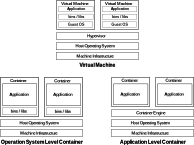
\includegraphics[width=\textwidth]{graphics/virtualization.svg}
    \caption{\textit{Virtual Machines} compared to Operation System Level and Application Level \textit{Containers}~\cite{docker1}}
    \label{fig:container_levels}
\end{figure}

\begin{itemize}
    \item[]{\textbf{Operation System Level Container}\\
    Encapsulates its own operation system while sharing the kernel with other \textit{Containers} on the host.}
    \item[]{\textbf{Application Level Container}\\
    Incorporates all processes an application needs to run while sharing the operation system with other \textit{Containers} on the host.}
\end{itemize}
Containerization enables many advantages over traditional virtualization.
Since \textit{Containers} are much more lightweight than \textit{Virtual Machines} it is possible to operate more containers on a computing resource.
Additionally the initialisation is almost instant compared to the protracted booting process of a \textit{Virtual Machine}.
Further \textit{Containers} are much more portable because all libraries and dependencies are encapsulated and can be operated regardless of the underlying operating system of the host machine~\cite{docker2, docker1, virt1}.

\section{Microservices}
The growing popularity of small applications that are packaged in a single container led to a new paradigm in software architecture.
Within a typical \textit{Microservice} based architecture there exist many standalone services which collaborate through one or more network endpoints to reach a defined business goal together.
The key characteristic of those services is that each is independently deployable, modeled around a business domain and technology agnostic.
That means that every \textit{Microservice} can be implemented with its own technology, data structure and even programming language.
Further while deploying changes of a \textit{Microservice} into production it should not be necessary to interact with other services.
To ensure this property all services need to be \textit{loosely coupled} which means that each component of a system can be changed or swapped independently.
This can be achieved through stable, explicit and well defined interfaces.
Additionally the borders of each service are not defined by expert groups of certain fields like backend, frontend or databases but by business domain. 
That means that there is a team with multiple skills in a company which develops a service that handles all details to reach one business goal.
For example a Team which has responsibility of a \textit{Microservice} which handles the payments of a \textit{SaaS} application.
The team implements and maintains all service components that the customer interacts with while conducting the payment process.
In this way the service contains a small part of user interface, a small part of application logic and a small part of data storage.
This principle reduces changes in different layers of an application across multiple teams and therefore enables organizations to ship changes and updates faster.
Another principle of \textit{Microservices} is the ownership of the data it operates with and therefore no indirect access of information through sharing databases.
That means that whenever a service needs data owned by another service it needs to explicitly ask the other service over a communication channel to pass on the desired information.
That concept facilitates a service to decide which data is shared with which external services.
It further allows to hide implementation details which can change for arbitrary reasons behind exposed stable service interfaces.
This brings the benefit of independently deployable \textit{Microservices} which do not induce adjustments to multiple services whenever a service changes its internals.
\\
\\
One of the key advantages of a \textit{Microservice} architecture is the independence of the various teams of a organization.
It allows teams to choose the technology which is best for achieving one specific business goal and find the optimal composition of programming languages, frameworks, databases and many more.
Further the independent deployability enables applications with a higher flexibility, availability, resiliency and scalability.
\\
\\
There are also potential pitfalls of using \textit{Microservices}.
One is that they depend on reliable network communication which is inherently slower than on a monolithic system.
Additionally varying latencies, packet loss and random connectivity issues can make the behavior of a whole \textit{Microservice} architecture unpredictable.
Another organisational pitfall is switching to \textit{Microservices} without having thought about the necessary groundwork.
The most important considerations are containerisation of applications, continuous integration and continuous delivery.
This fundamental automation prevents the organisation from ending up with many "mini monoliths" that need manual maintenance
Nevertheless managing a large amount of \textit{Microservices} across different cloud environments is still a complex task even when automated~\cite{Microservices1, Microservices2}.

\section{Orchestrating Containers within a Microservice Architecture}
Enterprise-level applications utilizing the \textit{Microservice} architecture are oftentimes made up of hundreds of containerized services that need to be orchestrated.
To provide a real customer value while optimizing provider costs this cluster of \textit{Containers} needs to be reliable and potentially globally available while making ideal use of computational resources.
To achieve this goal an orchestration engine aggregates a set of server hosts with its network connections into a single resource pool called cluster.
The engine autonomously deploys \textit{Containers}, schedules them across the cluster while scaling its number proportionally to the currently accruing workload to ensure defined policies and service level agreements are met~\cite{Microservices2, Orch1}.
~\cref{fig:orch_levels} illustrates that the orchestrator serves as foundation for the application layer and typically consists of three layers which sit on top of the hardware, operating system and container runtime layers~\cite{Orch2}:
\begin{itemize}
    \item[]{\textbf{Resource Management}\\
    This layer takes care of the low level resources like computation, data storage and network.
    Its goal is to maximize the utilization of those resources while preventing conflicts by competing \textit{Containers}.
    }
    \item[]{\textbf{Scheduling}\\
    This layer is concerned with the efficient usage of cluster internal resources. 
    It gets its service requirements through configuration files supplied by an administrator.
    It is then decided where the application \textit{Containers} are placed in the cluster with respect to the number of needed replicas and co-location constraints to leverage the full potential of inter-process communication.
    It is further responsible to ensure that a \textit{Container} is running and therefore constantly checking their availability and if necessary restarting crashed \textit{Containers}, move \textit{Containers} from failed nodes as well as scaling up the number of \textit{Containers} to deal with increasing workloads.
    }
    \item[]{\textbf{Service Management}\\
    The final layer allows administrators to define and manage the high level aspects of the underlying cluster like attaching meta data to \textit{Containers} and divide incoming traffic to balance workloads.
    Additionally it allows \textit{Container} isolation through the specification of \textit{namespaces}.
    This allows the cluster to be used by multiple tenants without interference.
    }
\end{itemize}
\begin{figure}[]
    \centering
    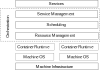
\includegraphics[width=0.6\textwidth]{graphics/orch_layers.svg}
    \caption{The Different Layers of Container Orchestration~\cite{Orch2}}
    \label{fig:orch_levels}
\end{figure}

\section{OpenStack}
The following section describes \textit{OpenStack} as Infrastructure as a Service solution which is needed as the groundwork for a scalable cloud environment.
It is an open source \textit{IaaS} platform written in python and developed by the National Aeronautics and Space Administration and RackSpace and published in 2010.
The OpenStack architecture consists of three main components: compute, image and storage.
There are many additional components in the OpenStack ecosystem which are out of scope for this thesis but some important will be mentioned briefly~\cite{open_stack, open_stack2}:
\begin{itemize}
    \item[]{\textbf{Compute}\\
    The \textit{Nova} component contains all tools to manage virtual machines on physical computing nodes and is used to administrate \textit{IaaS Clouds}.
    It provides an external communication channel to applications or administrators through an API server.
    It handles the orchestration and life cycle of instances by creating and managing virtual servers without a strict dependency on a \textit{Hypervisor}.
    Additionally it includes tools to manage networks as well as access control and serves as an essential building block for a basic \textit{Cloud Computing} implementation.
    }
    \item[]{\textbf{Image}\\
    This component also known as \textit{Glance} serves as a central catalog for \textit{VM} images.
    It allows discovery, preservation and retrieval of images based on metadata.
    }
    \item[]{\textbf{Object}\\
    \textit{Swift} is a redundant and scalable component to manage an object store.
    It provides users with storage capacity in a highly distributed architecture to prevent data loss through single points of failure.
    }
    \item[]{\textbf{Additional Components}
    \begin{itemize}
    \item[]{\textbf{Horizon:} Is a dashboard to monitor, manage and provision services in \textit{OpenStack}.}
    \item[]{\textbf{Keystone:} Supplies an authentication service to apply tokens and policies to users and service interactions.
    It is an essential service to provide \textit{Cloud} services to end users.}
    \item[]{\textbf{Cinder:} Enables persistent volumes to virtual machines and was encompassed in \textit{Nova} in previous releases.
    It uses the \textit{Swift} component as backup for the supplied persistent volumes.
    }
    \item[]{\textbf{Neutron:} Is a service which provides network connectivity and allows the configuration of advanced network topologies and policies.}
    \end{itemize}
    }
\end{itemize}

\subsection{Alternative Infrastructure-as-a-Service Technologies}
The following alternative solutions for Infrastructure-as-a-Service were also examined and compared to OpenStack:
\begin{itemize}
    \item[]{\textbf{Apache Cloud Stack}\\
    This open source platform is implemented in Java, was originally released by Cloud.com in 2010 and was donated to the Apache Incubator in 2012 and has since then become a top-level project of the Apache Software Foundation.
    \textit{Apache Cloud Stack} consists of three nodes a \textit{Supervisor Node}, a \textit{VM Creator Node} and a \textit{StorageServer Node} which is for the most part identical with \textit{OpenStack}.
    The main differentiator from \textit{OpenStack} is that it is easier to configure since it is not made up of a collection of separately configurable components.
    This implies a lower flexibility when it comes to highly complex deployment scenarios.
    A further disadvantage which is crucial for this thesis is the lack of native \textit{Docker} support~\cite{cloud_stack, cloud_stack2}.
    }
    \item[]{\textbf{OpenNebula}\\
    \textit{OpenNebula} is a platform for managing distributed infrastructures mainly in large scale data centers and was released in 2008.
    It is primarily implemented in C++ as well as Ruby, utilizes the Linux native drivers concept and consists of three layers.
    The \textit{Drivers Layer} communicates with the underlying operating system and abstracts the infrastructure of the host as a set of services.
    The middle layer is concerned with managing the \textit{Virtual Machines} and their networks and is called \textit{Core Layer}.
    The final \textit{Tool Layer} contains interfaces that allow for user interaction as well as the scheduling of \textit{VMs}~\cite{open_nebula, open_nebula2}.
    }
\end{itemize}
The primary reason to chose \textit{OpenStack} is that the university department at which this thesis was conducted already operates an instance and has the experience to provide the required infrastructure in a stable and reliable manner.

\section{Docker}
The following section describes \textit{Docker} as lightweight container virtualization technology of choice because its wide popularity and the many available images from large organizations.
It is capable of creating, deploying and managing containerized applications and was created by Docker Inc. in 2013.
To use \textit{Docker} a \textit{Image} is necessary.
It is a file which contains all specifications needed to create a \textit{Container}.
Usually an \textit{Image} contains another base \textit{Image} with additional customization which is required to successfully operate an application.
A \textit{Container} describes instance based on an \textit{Image} which can be started, stopped, moved or deleted.
\textit{Docker} consist of two main parts the \textit{Runtime} and the \textit{Daemon} sometimes called engine~\cite{docker2}:
\begin{itemize}
    \item[]{\textbf{Runtime}\\
    The overall runtime is responsible for setting up the environment like \textit{cgroups} and \textit{namespaces} as well as starting and stopping containers.
    It consists of high-level and low-level runtime which communicate with each other.
    The low-level one is called \textit{runc}, is part of every container and forms the interface to the underlying operating system to start and stop the \textit{Container}.
    The high-level \textit{Runtime} \textit{containerd} interferes with \textit{runc} and manages the whole lifecycle of a \textit{Container} as well as pulling \textit{Images} and assembling network interfaces.
    }
    \item[]{\textbf{Daemon}\\
    The \textit{Docker engine} also known as \textit{dockerd} was created to abstract both levels of the \textit{Runtime} and provide a swift interface.
    It communicates with \textit{containerd} and enables \textit{Image}, networking and volume management.
    \textit{dockerd} also exposes the \textit{Docker} API to establish a channel of interaction.
    }
\end{itemize}

\subsection{Alternative Container Virtualisation Technologies}
The following alternative solutions for \textit{Container} virtualisation technologies were also examined and compared to \textit{Docker}:
\begin{itemize}
    \item[]{\textbf{Podman}\\
    \textit{Podman} was designed to leverage Linux native components to a deamonless \textit{Container} technology.
    That means that \textit{Podman} is independent on a single \textit{Deamon} process which may pose as a single point of failure.
    Instead it is directly interacting with the \textit{runc} container runtime.
    It is able to run, build and deploy containerized applications or images that are compliant with the \textit{Open Containers Initiative (OCI)} standards.
    Hence \textit{Podman} is able to manage containers build in \textit{Docker}.
    Additionally the processes controlled by \textit{Podman} can be run as \textit{root} or as \textit{unprivileged user}.
    Whereas the \textit{Docker deamon} requires to be executed as \textit{root} which can lead to security implications~\cite{podman}.
    Since there is not a large developer community nor much literature available for \textit{Podman} it was not further considered for this thesis.
    }
    \item[]{\textbf{LXC}\\
    \textit{LinuX Containers} enhances the \textit{cgroups} as well as the \textit{namespaces} functionality of the Linux kernel to provide a contained environment to execute applications.
    It is maintained by Canonical Inc. which is also responsible for the \textit{Ubuntu} Linux distribution and was released in 2008.
    In contrast to \textit{Docker} which handles application level containers \textit{LXC} manages operation level containers~\cite{lxc, docker1}.
    The difference between both technologies is illustrated in~\cref{fig:container_levels}.
    Since \textit{LXC} have no native support in Kubernetes they are not examined further.
    }
    \item[]{\textbf{FreeBSD Jails}\\
    \textit{Jails} are one of the earliest attempts to realize things like process isolation dating back to the year 2000.
    To achieve this the BSD kernel feature \textit{croot} was further customized to virtualize file access, system users and the networking subsystem.
    This allows multiple processes to utilize those virtualized resources while having only restricted access to a subset of the whole file system.
    Each \textit{Jail} contains a set of users and a root which are limited to their own environment~\cite{jails}.
    Like \textit{LXC} the concept of \textit{FreeBDS Jails} can be classified as a operating system level container.
    Since it is only available on the \textit{FreeBSD} distribution this technology is out of scope for this thesis.
    }
\end{itemize}
\textit{Docker} was chosen for this thesis since it has an extensive documentation, a large developers community and has been the de facto standard container runtime used by Kubernetes.
Additionally the related work which is fundamental for this thesis was conducted using \textit{Docker}.

\section{Kubernetes}
The following section describes \textit{Kubernetes} which is a container orchestration system that allows the operation of scalable applications with changing topologies based on workload or traffic.
It was primarily developed as an internal project at Google to manage large containerized applications like Gmail and was open sourced in 2015.
\textit{Kubernetes} is organized in a Master-Slave architecture with the master node controlling all Minion computing nodes and consists of the following componenents~\cite{KUB, KUB4}:
\begin{itemize}
    \item[]{\textbf{Master Node}\\
    The \textit{Master Node} also known as \textit{Control Plane} controls the operations inside the cluster.
    It is concerned to manage the distribution of \textit{Pods} between the available \textit{Minion Nodes}.
    To extend the robustness of the system it is possible to create multiple redundant \textit{Master Nodes}.
    The \textit{Control Plane} utilizes the following processes and components:
    \begin{itemize}
    \item[]{\textbf{API Server: }Serves as the main interaction point of the cluster.
    It receives \textit{JSON} formatted configurations over a \textit{REST} API and stores them in \textit{etcd}.
    }
    \item[]{\textbf{etcd: }Is a lightweight distributed \textit{Key-Value-Database} which preserves the configured target state of the cluster.
    }
    \item[]{\textbf{Controller Manager: }Is an independent component which runs all controller processes and communicates with the \textit{API Server} regarding the status of the cluster.
    It observes whether all nodes are available and all pods were launched correctly.
    Further it populates the \textit{Endpoints} object and thus connects \textit{Services} and \textit{Pods}.
    }
    \item[]{\textbf{Scheduler: }Decides on which \textit{Minion Nodes} a \textit{Pod} is deployed and is constrained by specifications of quality of service, node locations and available resources.
    Additionally it is concerned with the management and overseeing of the workload directed to the \textit{Minion Nodes}.
    }
    \end{itemize}
    }
    \item[]{\textbf{Minion Node}\\
    A \textit{Minion Node} describes a single host machine that is used by \textit{Kubernetes} to form a large scale cluster.
    Each node contains a container runtime as well as the following components:
    \begin{itemize}
    \item[]{\textbf{Kubelet: }Is responsible for the state of all \textit{Pods} on a particular host machine and communicates its state to the \textit{Control Manager} on the \textit{Master Node}.
    \textit{Kubelet} undertakes the restart of a failed \textit{Pod} on the same machine.
    If the communication between \textit{Kubelet} and \textit{Control Plane} is interrupted the \textit{Master Node} assumes a failed node and moves all its \textit{Pods} onto an available host machine.
    }
    \item[]{\textbf{cAdvisor: }Records the utilization of the resources of a \textit{Minion Node} and can be accessed by external applications to provide dynamic scaling of the whole cluster.}
    \item[]{\textbf{Kube-Proxy: }Manages the connections and open ports on a node}
    \end{itemize}
    }
\end{itemize}

\subsection{Alternative Container Orchestration Systems}
The following alternative solutions for container orchestration systems were also examined and compared to \textit{Kubernetes}:
\begin{itemize}
    \item[]{\textbf{Docker Swarm}\\
    \textit{Docker Swarm} is an open source project by Docker Inc. to provide native cluster management support in \textit{Docker}.
    It bundles several \textit{Docker} nodes into one cluster to enable dynamic scaling as well as a failover mechanism through redundancy.
    Like \textit{Kubernetes} it is organized in a master-slave architecture where the master is called \textit{Manager} and accounts for the orchestration of \textit{Containers}.
    The slave is known as \textit{Agent} which operates the scheduled \textit{Containers}.
    Compared to \textit{Kubernetes} it is far less feature rich in both \textit{Scheduling} and \textit{Service Management Layers}.
    \textit{Docker Swarm} lacks the support of readiness checking and rolling deployments which can lead to data loss and impacts on the availability of a service.
    Further it does not support \textit{namespaces} and \textit{load balancing} that means that no multi tenancy and no dynamic traffic distribution is available in a \textit{Docker Swarm} cluster.
    Since \textit{Kubernetes} supports all those features that are particularly important for an Enterprise Content Management System \textit{Docker Swarm} is not further considered~\cite{docker2, Orch2}.
    }
    \item[]{\textbf{Apache Mesos}\\
    Hello Test
    \textit{Apache Mesos} is an open source project developed by the University of California, Berkeley in 2011 which follows the master-slave architecture pattern.
    \textit{Master Nodes} control \textit{Slave Nodes} that contain \textit{Frameworks} which execute \textit{Tasks}.
    The \textit{Master Node} decides based on specified \textit{Policies} how many free resources are assigned to each \textit{Framework}.
    A \textit{Framework} contains a \textit{Scheduler} which communicates with the \textit{Master Node} to allocate computing resources and an \textit{Executor} that completes \textit{Tasks} on a \textit{Slave Node}.
    Compared to \textit{Kubernetes} it contains slightly more features in the \textit{Resource Management} and \textit{Service Management Layers} however the one major disadvantage is the rather complex setup and integration of applications.
    \textit{Apache Mesos} requires \textit{Marathon} to be installed on top of it to support containerized workloads.
    ~\cite{mesos, Orch2}
    }
    \item[]{\textbf{OpenShift}\\
    \textit{OpenShift} is Red Hat's own \textit{Kubernetes} distribution which is fully compliant and extends it with features focused on improving the productivity of developers and operators.
    It was originally released with an own runtime environment in 2011 and later rewritten to implement \textit{Kubernetes} in 2015.
    The proprietary features contributed by Red Hat improve the native networking and provide support in the life cycle of deployed images~\cite{Openshift}.
    Since \textit{OpenShift} is not entirely open source and the additonal functionality is not relevant for this thesis it was not further considered.
    }
\end{itemize}
Kubernetes posed as an excellent choice since it is entirely open source, implements the right balance of required features and operational complexity.
Further it has the largest market adaption among orchestration systems and therefore a large developer community and many learning resources.